% Ward Vitals Pipeline: EC8203 mini-project report.
% Build: pdflatex main.tex (twice, for page references) or upload this folder to Overleaf.
% Screenshots: put the PNG in figures/ with the name used in \shot{...}; until then a placeholder is shown.
\documentclass[11pt,a4paper]{article}

\usepackage[utf8]{inputenc}
\usepackage[T1]{fontenc}
\usepackage{lmodern}
\usepackage{microtype}
\usepackage[a4paper,left=2.3cm,right=2.3cm,top=2cm,bottom=2.2cm]{geometry}
\usepackage{graphicx}
\usepackage[table]{xcolor}
\usepackage{tabularx}
\usepackage{array}
\usepackage{booktabs}
\usepackage{enumitem}
\usepackage{caption}
\usepackage{titlesec}
\usepackage{fancyhdr}
\usepackage{lastpage}
\usepackage{textcomp}
\usepackage{float}
\usepackage[hidelinks]{hyperref}

\graphicspath{{figures/}}

% ------------------------------------------------------------------ colours --
\definecolor{navy}{HTML}{1F3864}
\definecolor{blue2}{HTML}{2E5597}
\definecolor{grey}{HTML}{555555}
\definecolor{head}{HTML}{DCE6F2}
\definecolor{rule}{HTML}{BFBFBF}
\definecolor{shotbg}{HTML}{EAF1FB}
\definecolor{shotfg}{HTML}{1F4E79}

% ------------------------------------------------------------------- layout --
\setlength{\parindent}{0pt}
\setlength{\parskip}{4pt}
\linespread{1.0}
\setlength{\tabcolsep}{4pt}
\titleformat{\section}{\large\bfseries\color{navy}}{}{0pt}{}
\titleformat{\subsection}{\normalsize\bfseries\color{blue2}}{}{0pt}{}
\titlespacing*{\section}{0pt}{10pt}{4pt}
\titlespacing*{\subsection}{0pt}{7pt}{3pt}
\setlist{nosep,leftmargin=1.4em,topsep=2pt}
\captionsetup{font={small,it},labelfont={small,it},textfont={color=grey},skip=4pt}

\pagestyle{fancy}
\fancyhf{}
\renewcommand{\headrulewidth}{0pt}
\cfoot{\footnotesize\color{grey}Page \thepage\ of \pageref*{LastPage}}

% ------------------------------------------------------------------ helpers --
% Code in running text; may break after an underscore.
\newcommand{\ubreak}{\textunderscore\allowbreak}
\newcommand{\code}[1]{{\small\ttfamily\let\_\ubreak #1}}
\newcommand{\spo}{SpO\textsubscript{2}}
\newcommand{\degC}{\,\textdegree C}
% Screenshot slot: image if figures/#1 exists, otherwise a shaded placeholder.
\newcommand{\shot}[2]{%
  \IfFileExists{figures/#1}{%
    \begin{figure}[H]\centering\includegraphics[width=0.9\linewidth]{#1}\caption{#2}\end{figure}}{%
    \par\smallskip\noindent\colorbox{shotbg}{\parbox{\dimexpr\linewidth-2\fboxsep}{\centering
      \small\itshape\color{shotfg}[Insert screenshot: #2 \,$\rightarrow$\, figures/\detokenize{#1}]}}\par\smallskip}}

% Tables: small type, header shading, grey rules, ragged cells.
\newcolumntype{L}[1]{>{\raggedright\arraybackslash}p{\dimexpr#1\linewidth-2\tabcolsep-1pt\relax}}
% Optional argument: font size (default \small).
\newenvironment{rtable}[2][\small]
  {\par\smallskip#1\arrayrulecolor{rule}\renewcommand{\arraystretch}{1.15}%
   \noindent\begin{tabular}{|#2|}\hline\rowcolor{head}}
  {\\\hline\end{tabular}\par\smallskip}
\newcommand{\tcap}[1]{\vspace{-4pt}\captionsetup{hypcap=false}\captionof{table}{#1}}

\begin{document}

% ================================================================ cover page ==
\begin{titlepage}
\centering
\vspace*{2.2cm}
{\color{grey}\large EC8203 Applied Big Data Engineering\par}
\vspace{2pt}
{\color{grey}Mini-project report \textperiodcentered{} Use case 2: Hospital Patient Vital Signs Monitoring\par}
\vspace{2.4cm}
{\color{navy}\bfseries\fontsize{28}{34}\selectfont Ward Vitals Pipeline\par}
\vspace{10pt}
{\color{blue2}\Large A Lambda Architecture for Near-Real-Time Patient Monitoring\par
with Daily Lab-Result Consolidation\par}
\vspace{2.2cm}
\begin{rtable}{L{0.113}|L{0.180}|L{0.698}}
\textbf{Member} & \textbf{Name} & \textbf{Slice} \\\hline
A & Ninada & Real-time vitals: producer, Kafka, streaming windows, trend \\\hline
B & Imalsha & Labs and history: lab feed, lake, risk rules, Airflow, risk join, report \\\hline
C & Kasun & Alerts, serving and observability: alert rules, API, monitoring
\end{rtable}
\vspace{0.8cm}
{\color{grey}\small Repository: \textless URL\textgreater \quad\textperiodcentered\quad Demo video: \textless link\textgreater\par
\vspace{3pt}Submitted 5 October 2026\par}
\vspace{1.6cm}
\begin{minipage}{0.8\linewidth}
{\color{navy}\bfseries Contents}\par\vspace{4pt}
\small
\begin{tabular}{@{}l@{\hspace{10pt}}l@{}}
1 & Introduction \\ 2 & Business requirements \\ 3 & Architecture decision: Lambda vs Kappa \\
4 & Architecture \\ 5 & Technology stack and justification \\ 6 & Data design \\
7 & Processing (7a streaming, 7b batch) \\ 8 & Storage and serving (8a storage, 8b serving) \\
9 & Observability \\ 10 & Results \\ 11 & Limitations, trade-offs and production scale \\
12 & Conclusion \\ & Individual contributions
\end{tabular}
\end{minipage}
\vfill
{\color{grey}\small\itshape Risk thresholds in this project are simulated rules for a data-engineering exercise.
They are not clinical guidance.\par}
\end{titlepage}

% ========================================================================= 1 ==
\section{1. Introduction}
A hospital ward monitors patients through bedside sensors that report vital signs every few seconds, while the
pathology lab publishes blood-test results once a day. The two only make sense together: a raised heart rate means
more when the same patient's lactate is high. This project builds a data platform that ingests both sources,
processes the stream in near real time, joins it daily with the lab results, and serves the combined picture
through an API, a daily report and a monitoring dashboard.

The system is an end-to-end \textbf{Lambda architecture} on Apache Kafka, Apache Spark (Structured Streaming and
batch), Apache Airflow, a Parquet data lake and PostgreSQL, with Prometheus and Grafana for observability, all
started from one Docker Compose file. \S3 argues the architecture decision, \S4--\S8 present the design, \S9 how
the running system is observed, \S10 what it produces, and \S11 where it falls short of production.

% ========================================================================= 2 ==
\section{2. Business requirements}
\textbf{Use case 2: Hospital Patient Vital Signs Monitoring.} Fifteen patients wear bedside monitors that report
heart rate, \spo, blood pressure and temperature every 2--5\,s; once a day the pathology lab delivers a file of
results. The ward asks: \emph{which patients show concerning vital-sign trends right now} (seconds matter), and
\emph{how do yesterday's lab results change the risk picture} (once a day)? We read these as the requirements below.

\begin{rtable}{L{0.052}|L{0.36}|L{0.283}|L{0.295}}
\textbf{\#} & \textbf{Requirement} & \textbf{Met by} & \textbf{Result} \\\hline
R1 & Live ward view: each patient's vitals, trend and risk within seconds & Q1 $\rightarrow$ \code{patient\_current\_status} $\rightarrow$ API & 6.2\,s average reading-to-table, 9\,s worst \\\hline
R2 & Per-patient alerts, stronger when a limit stays broken & Q3 $\rightarrow$ \code{patient-alerts} $\rightarrow$ \code{vital\_alerts} & P007 spike: CRITICAL alert via the API \\\hline
R3 & Trends, not only single values & Q1 trend over three windows & \spo{} drop marked FALLING after 75\,s \\\hline
R4 & Daily lab feed, loaded completely or not at all & Lab DAG (\S7b) & 80 of 80 rows loaded; a bad file rejected \\\hline
R5 & Daily consolidated risk: vitals + newest labs & Risk join and report (\S7b, \S10) & Labs moved 3 patients to CONCERNING \\\hline
R6 & Queryable serving: live and merged views & FastAPI (\S8b) & \\\hline
R7 & Recompute past days after a rule change & Parquet lake + batch jobs & Re-running a day gives identical rows \\\hline
R8 & Invalid readings kept out of the view but kept for diagnosis & Validation, DLQ, de-duplication & 17 malformed events quarantined \\\hline
R9 & Observable pipeline: logs, metrics, health alerts & \S9 & 15 alert rules
\end{rtable}

\textbf{Risk model (project-defined).} Per 2-minute window (speed layer) or per day (batch layer): \spo{} minimum
$<$\,92\,\% scores +2; heart-rate average outside 50--120\,bpm +1; temperature maximum $>$\,38.0\degC{} +1;
systolic pressure outside 90--160\,mmHg +1; heart rate rising or \spo{} falling over three consecutive windows +1
(speed layer). Each lab result outside its reference range scores +1, or +2 beyond 1.5$\times$ the limit. The total
maps to \textbf{NORMAL} (0--1), \textbf{WATCH} (2--3) or \textbf{CONCERNING} ($\geq$\,4). A patient without recent
labs is \textbf{LAB\_UNAVAILABLE}, never a lab score of 0.

\textbf{Assumptions.} One simulated day lasts \textbf{300 real seconds}, so ``yesterday's labs'' are five minutes
old. The system runs on one machine with a single Kafka broker; \S11 lists what changes at production scale.

% ========================================================================= 3 ==
\section{3. Architecture decision: Lambda vs Kappa}
\textbf{Decision: Lambda.} A speed layer (Spark Structured Streaming) answers the first question from the vital
stream. A batch layer (Airflow and Spark batch) answers the second by recomputing daily views from an immutable
master dataset and the lab file. The serving layer merges them. \textbf{Kappa is the rejected alternative.}

\textbf{The two candidates.} In our \emph{Lambda} design every reading goes to Kafka; three streaming queries read
it: Q1 (live view), Q3 (alerts) and Q2, which archives every event to a Parquet lake partitioned by simulated day.
Once a day Airflow waits for the lab file, loads it, recomputes the day's vital summary from the lake and joins it
with the newest labs. In \emph{Kappa}, Kafka's log would be the only source of truth: the lab file would be
published to a \code{lab-results} topic, and one streaming job would compute both the live view and a day-long
per-patient window joined with the lab stream. Changing a rule would mean replaying the topics through a new job
version.

\begin{rtable}{L{0.213}|L{0.389}|L{0.389}}
\textbf{Criterion} & \textbf{Lambda (built)} & \textbf{Kappa (rejected)} \\\hline
\textbf{Latency}: live view in seconds, daily view once a day & Speed layer: 6.2\,s average reading-to-table. Daily view ready 1--2\,min after the day ends. & Same live latency. The daily view can update during the day, but is only final when the day's window closes. \\\hline
\textbf{Replay}: recompute any past day after a rule change & The lake keeps every raw event indefinitely. Day N is recomputed from one partition; the summary job takes $\sim$43\,s and gives identical rows on a re-run. & Bounded by Kafka retention (7 days here) unless the broker becomes the long-term store. The lab file is not in Kafka at all without an extra topic. \\\hline
\textbf{Consistency}: daily risk complete and repeatable; live view may approximate & The batch view counts every event, including readings too late for the 1-minute watermark. Days are replaced atomically. & One code path, so no drift. But a reading later than the watermark is lost for good unless state is held longer. \\\hline
\textbf{Cost}: small team, two weeks, one laptop & Two processing paths to build and run; logic duplication contained by one shared rules module. The batch path runs once per day. & One codebase and runtime, but a day of state per patient for the join, and every reprocessing replays the whole topic.
\end{rtable}

\textbf{Why Lambda fits this use case.}
\begin{enumerate}
\item \textbf{Half the data is a daily file.} A lab file is complete only when all of it has arrived, can be late or
  missing, and must be rejected as a whole when bad. Airflow's sensor, validation, retries and failure callbacks
  model this directly; in Kappa a streaming job would have to rebuild ``the file for day N is complete'', which is
  the batch layer again.
\item \textbf{The question has two time scales.} The live question needs seconds and tolerates approximation; the
  daily report is acted on and must be complete and repeatable. Lambda gives each its own path with the right
  trade-off.
\item \textbf{Replay beyond Kafka retention.} Monitoring rules change, and past days must then be recomputed. The
  partitioned lake makes that a read of one folder, independent of Kafka retention.
\item \textbf{The brief asks for orchestrated historical reporting}, which is the batch layer; Kappa would still
  need a scheduler for the report.
\end{enumerate}

\textbf{When Kappa would win.} If lab results arrived as individual events (e.g.\ HL7 messages as each test
finishes), with long retention or tiered storage available and budget for only one runtime, the second path would
buy little. The brief fixes the lab source as a daily file, so that is not our case.

\begin{rtable}{L{0.224}|L{0.319}|L{0.447}}
\textbf{Lambda weakness} & \textbf{How it shows here} & \textbf{Mitigation} \\\hline
Logic written twice drifts apart & ``Abnormal'' and ``risk'' are needed in Q1, Q3, the daily summary, the risk join and the API & One rules module from one \code{thresholds.yaml}, in Python and Spark forms, with parity tests (\S7b); Q2 and the summary reuse Q1's parser and abnormal check \\\hline
Two answers to one question & Live risk from a 2-minute window, daily risk from the whole day & Both shown and labelled by source: the API returns the speed and batch views separately \\\hline
More moving parts & Kafka, Spark streaming and batch, Airflow, PostgreSQL & One Compose file with pinned versions; health alerts per layer (\S9) \\\hline
Layers compete for one machine & On a 4\,GB laptop a daily run sometimes exceeded one simulated day & Each Spark app capped at 2 cores; the DAG skips ahead instead of queueing
\end{rtable}

% ========================================================================= 4 ==
\section{4. Architecture}
Figure~\ref{fig:arch} shows every component by layer and owner. Three choices shape it: \textbf{one master
dataset} (Q2 archives every event, including invalid ones, and the batch layer reads only the lake, never Kafka);
\textbf{one rule set for both layers} (\code{common/risk\_rules.py}); and \textbf{files handed over by contract, not
by timing} (the lab file is written atomically, then a \code{\_SUCCESS} marker that Airflow waits for).

\begin{figure}[H]
\centering
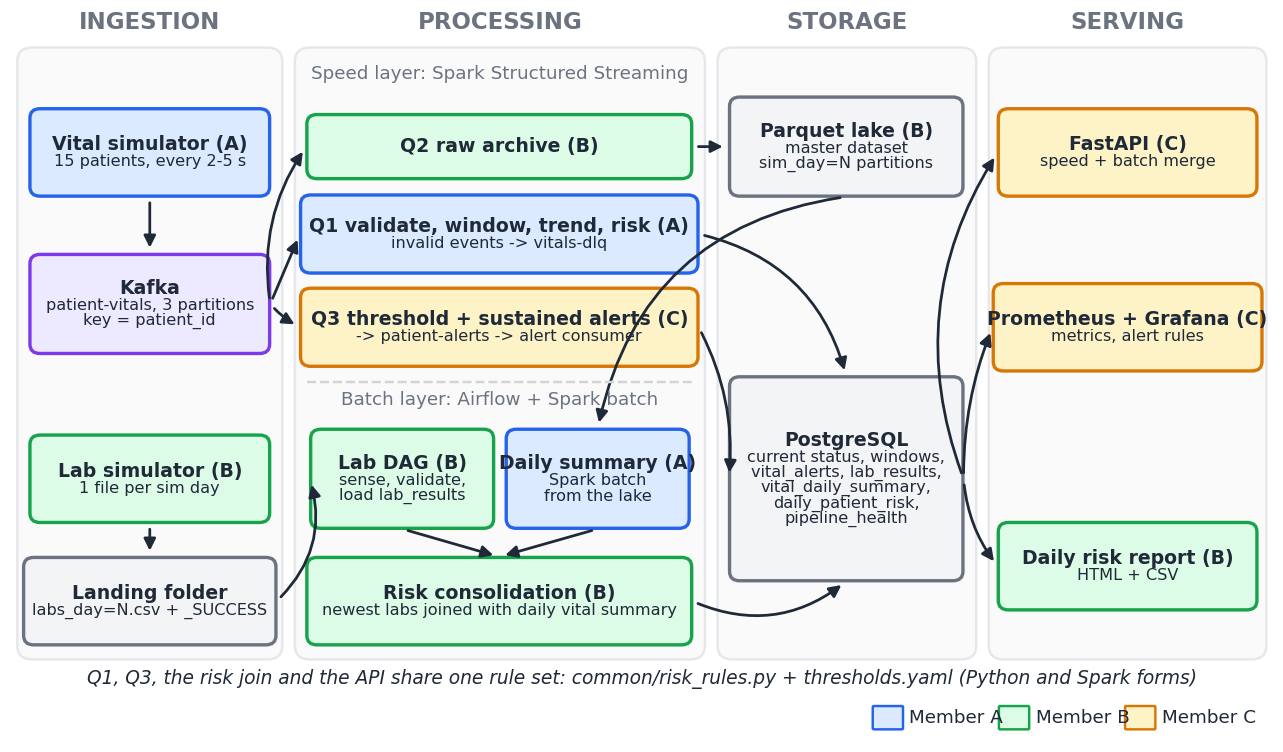
\includegraphics[width=\linewidth]{fig_architecture.png}
\caption{Component architecture across ingestion, processing, storage and serving.}
\label{fig:arch}
\end{figure}

\textbf{Simulated clock.} Every component computes \code{sim\_day = floor((t $-$ SIM\_EPOCH) / 300)} through the
shared \code{common/sim\_clock.py}, from event time, never arrival time, with the epoch and day length read from one
configuration (\code{config/app.yaml}, overridden by \code{.env}). A reading from 23:59:59 of a day belongs to that
day even if processed after midnight.

\textbf{One simulated day, end to end.} When day N ends, the lab simulator writes \code{labs\_day=N.csv} and its
marker; Airflow's sensor sees the marker, validates the file and loads \code{lab\_results}. Once Q2 has committed
the day's last readings, Spark recomputes the day's vital summary from the lake, joins it with the newest labs into
\code{daily\_patient\_risk}, and the report is written. Independently, the speed layer updates each patient's status
within about 10\,s of every reading.

\textbf{Deployment.} One Docker Compose file with pinned versions: Kafka 3.9 (KRaft), Spark 3.5.5 standalone (one
master, one 4-core worker), Airflow 2.10.5 (LocalExecutor), PostgreSQL 16, FastAPI, and a \code{monitoring} profile
with Prometheus, Pushgateway, kafka-exporter and Grafana. The streaming application and each batch job are capped
at 2 cores so they fit side by side; Airflow submits Spark jobs in client mode.

% ========================================================================= 5 ==
\section{5. Technology stack and justification}
\begin{rtable}{L{0.138}|L{0.213}|L{0.639}}
\textbf{Layer} & \textbf{Choice} & \textbf{Why it fits this use case} \\\hline
Ingestion & \textbf{Apache Kafka 3.9}, 3 partitions & Keying by \code{patient\_id} keeps each patient's readings in order while spreading patients over partitions; a durable, replayable log decouples bedside producers from processing; a DLQ topic holds invalid events. Writing straight to a database would give neither replay nor decoupling. \\\hline
Stream processing & \textbf{Spark Structured Streaming 3.5} & Event-time windows with watermarks, de-duplication within the watermark, an exactly-once file sink and \code{foreachBatch} for idempotent upserts. The same engine runs the batch jobs, so rules are written once as Spark expressions; Storm would need a second engine and a second copy of the rules. \\\hline
Batch processing & \textbf{Spark batch} & Partition pruning on the lake, JDBC to PostgreSQL, window functions for ``newest labs per patient''; scales beyond one ward where pandas would not. \\\hline
Orches\-tration & \textbf{Apache Airflow 2.10} & The lab source is a daily file: FileSensor, retries, failure callbacks, a schedule aligned to the simulated day, reruns by parameter and task logs. Cron offers none of these. \\\hline
Master dataset & \textbf{Parquet lake} by \code{sim\_day} & Columnar and compressed for scans of a few columns; one folder per day for pruning; immutable files make recomputation safe. \\\hline
Serving store & \textbf{PostgreSQL 16} & Small, query-heavy tables; transactions make ``replace day N'' atomic; \code{ON CONFLICT} upserts make streaming sinks idempotent; check constraints enforce data rules. Cassandra targets write scale we do not have and lacks transactions and joins. \\\hline
Serving and observability & \textbf{FastAPI}; \textbf{Prometheus, Pushgateway, kafka-exporter, Grafana} & Typed API with OpenAPI docs, testable with \code{TestClient}. Pull metrics for services, push for short-lived jobs, Kafka lag, alert rules and dashboard in version control. \\\hline
Packaging & \textbf{Docker Compose}, pinned tags & One command reproduces the system; pinned versions keep Spark, the Kafka connector and Airflow's \code{pyspark} identical.
\end{rtable}

% ========================================================================= 6 ==
\section{6. Data design}
\subsection{6.1 Vital-sign events and Kafka}
Each reading is one JSON object: \code{event\_id} (UUID, unique per reading and run), \code{patient\_id} (the Kafka
key), \code{bed\_id}, \code{heart\_rate}, \code{spo2}, \code{systolic\_bp}, \code{diastolic\_bp},
\code{temperature} and \code{timestamp} (ISO-8601 UTC event time). Physical plausibility limits (e.g.\ \spo{}
50--100) separate sensor errors, which go to the dead-letter topic, from clinical thresholds, which only mark a
valid reading as abnormal. The simulator gives each of 15 patients a seeded baseline with noise and 3\,\%
single-reading spikes, plus repeatable demo scenarios (\code{spike}, \code{hr\_spike}, \code{spo2\_drop},
\code{outage}; two runs with one seed raised the same 48 alerts within 4\,ms) and an optional share of deliberately
malformed events.

\begin{rtable}{L{0.192}|L{0.106}|L{0.138}|L{0.554}}
\textbf{Topic} & \textbf{Parti\-tions} & \textbf{Key} & \textbf{Written by $\rightarrow$ read by} \\\hline
\code{patient-vitals} & 3 & \code{patient\_id} & Producer $\rightarrow$ Q1, Q2, Q3 \\\hline
\code{vitals-dlq} & 1 & \code{patient\_id} & Q1 $\rightarrow$ operators (rejected readings with \code{reason}, raw payload, source offset) \\\hline
\code{patient-alerts} & 3 & \code{patient\_id} & Q3 $\rightarrow$ alert consumer (consumer group)
\end{rtable}

\textbf{Why the key is patient\_id.} Kafka orders messages only within a partition; windows, trends and sustained
alerts are all per patient, so per-patient order is the order that matters. The producer uses \code{acks=all},
idempotence with retries (a retried batch is written once), a 20\,ms linger and the murmur2 partitioner; its
delivery callback counts sent and failed messages and warns if a patient ever changes partition. In the observed
run the partitions held 8, 5 and 2 patients (66,581, 41,620 and 16,633 messages), every patient stayed on one
partition, and lag stayed at zero. Hashing 15 keys into 3 buckets is lumpy; with hundreds of patients it evens out.
Retention is 7 days; replication is 1 (single broker).

\shot{a_kafka_partitions.png}{Kafka UI, messages per partition of patient-vitals.}

\subsection{6.2 Daily lab file}
\code{labs\_day=N.csv} holds \code{patient\_id, test\_type, result\_value, unit, reference\_low, reference\_high,
collected\_at} for potassium, creatinine, haemoglobin, WBC, CRP and lactate. The brief's reference range is split
into low and high, so the range check is a comparison and the batch layer needs no lab catalogue. The file is
followed by \code{labs\_day=N.csv.\_SUCCESS}, a JSON marker with the row count. To exercise the pipeline, about
10\,\% of patients have no results on a day, 5\,\% of tests are missing and 12\,\% of results are out of range;
P007 always shows high CRP and lactate, matching the vitals demo. Each day's content comes from a seed derived from
the day number, so rewriting a day gives a byte-identical file.

% ======================================================================== 7a ==
\section{7. Processing}
\subsection{7a. Streaming (speed layer)}
One Spark application runs five streaming queries on \code{patient-vitals}, each with its own checkpoint so each
restarts exactly where it stopped: \code{q1\_windows} and \code{q1\_dlq} (Member A), \code{q2\_archive} (B) and
\code{q3\_threshold\_alerts} and \code{q3\_sustained\_alerts} (C).

\textbf{Q1: validate, window, trend, risk.}
\begin{itemize}
\item \textbf{Parse and validate.} \code{from\_json} with an explicit schema and a corrupt-record column. One
  \code{reason} expression checks, in order, malformed JSON, wrong type, missing or null fields, bad timestamp and
  implausible values; rejected events go to \code{vitals-dlq} with their raw payload. Nothing is dropped silently.
\item \textbf{Watermark and de-duplication.} Windows use event time. A 1-minute watermark bounds lateness and state:
  in the Spark UI state stays near 600 rows and the watermark gap near 70\,s.
  \code{dropDuplicatesWithinWatermark} on \code{event\_id} removes re-delivered readings; a streaming test confirms
  a duplicate counts once and a reading 3 minutes late changes no window.
\item \textbf{Sliding windows.} Per patient, 2-minute windows sliding every 30\,s compute the average, minimum and
  maximum of each vital plus reading and abnormal counts; two minutes hold 25--60 readings, enough to smooth noise
  while reacting within a minute. Output mode is update.
\item \textbf{Sink in one transaction.} \code{foreachBatch} upserts changed windows into
  \code{patient\_vital\_windows}, computes trend and risk, and upserts one row per patient into
  \code{patient\_current\_status}, guarded so an older window never replaces a newer one. With Kafka offsets in the
  checkpoint and only idempotent statements, a replayed batch leaves the tables unchanged: exactly-once results from
  an at-least-once sink.
\item \textbf{Trend.} A micro-batch sees only the windows it touched, so the last 10 minutes of windows are kept in
  \code{patient\_vital\_windows} and read back. Heart rate is RISING (\spo{} FALLING) when each of three consecutive
  windows moves that way by a minimum total change (5\,bpm, 1 \spo{} point), which stops noise making the trend
  flicker. In the \code{spo2\_drop} scenario P007 was marked FALLING 75\,s after the decline began.
\item \textbf{Risk.} Each current window is scored with the shared rules, including the trend point. In the
  \code{spike} scenario P007 rose to CONCERNING (4 points: low \spo, high heart rate, trend) with CRITICAL alerts
  from Q3.
\end{itemize}

\textbf{Q3: alerts.} Threshold alerts (WARNING) fire for any valid reading beyond a limit; sustained alerts
(CRITICAL) fire when the same limit is broken by at least 3 readings of one patient in a 1-minute tumbling window.
Because the Kafka sink is at-least-once, each alert has a deterministic \code{alert\_id} (event and rule, or
patient, rule and window start); the consumer commits Kafka offsets only after inserting with
\code{ON CONFLICT DO NOTHING}, giving effectively-once storage. Limits come from the same rules module as the risk
scores. \textbf{Q2} archives every event to the lake (\S8a), reusing Q1's parser.

\begin{table}[!htb]\centering
\begin{rtable}{L{0.296}|L{0.148}|L{0.171}|L{0.148}|L{0.228}}
\textbf{Query} & \textbf{Median batch} & \textbf{95th percentile} & \textbf{Max Kafka lag} & \textbf{Rows dropped by watermark} \\\hline
\code{q1\_windows} & 4.0\,s & 4.9\,s & 0 & 0 \\\hline
\code{q1\_dlq} & 0.9\,s & 1.6\,s & 0 & -- \\\hline
\code{q2\_archive} & 2.1\,s & 2.5\,s & 0 & -- \\\hline
\code{q3\_threshold\_alerts} & 1.4\,s & 1.8\,s & 0 & -- \\\hline
\code{q3\_sustained\_alerts} & 3.8\,s & 4.7\,s & 0 & 0
\end{rtable}
\tcap{Speed-layer micro-batches over 30 minutes (180 per query, 10\,s trigger; Q2 30\,s).}
\end{table}

Every batch finished well inside its trigger with zero lag, and \code{patient\_current\_status} was on average
6.2\,s (at most 9\,s) behind the reading's event time: the speed layer keeps up with the ward with room to spare.

\shot{a_spark_streaming.png}{Spark Structured Streaming tab with the five active queries.}

% ======================================================================== 7b ==
\subsection{7b. Batch (batch layer)}
One Airflow DAG, \code{daily\_lab\_consolidation}, runs once per simulated day and carries a lab file all the way to
the daily report (Figure~\ref{fig:dag}). Its schedule is every 300\,s from the epoch, so each run's data interval is
one simulated day: a scheduled run processes the day that has just ended, and a manual run with
\code{\{"sim\_day": N\}} processes or re-runs any day. With \code{catchup=False} and one active run, a run slower
than a day makes Airflow skip ahead instead of queueing.

\begin{figure}[H]
\centering
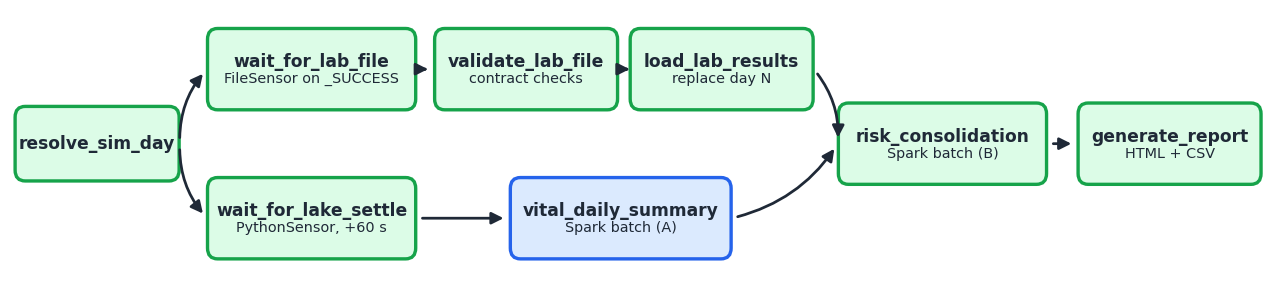
\includegraphics[width=\linewidth]{fig_dag.png}
\caption{The \texttt{daily\_lab\_consolidation} DAG: lab branch and vitals branch in parallel, joined by the risk
consolidation.}
\label{fig:dag}
\end{figure}

\begin{itemize}
\item \textbf{Sense.} A FileSensor waits for the \code{\_SUCCESS} marker, not the CSV. The simulator writes the CSV
  to a hidden temporary file, flushes it, renames it atomically and only then writes the marker, so a half-written
  file is never read. In \code{reschedule} mode the sensor frees its worker between checks; after two simulated days
  it fails (``lab file missing'').
\item \textbf{Validate.} Every row is checked against the contract shared with the simulator
  (\code{common/lab\_feed.py}): exact header; finite, non-negative numbers; known test type and patient id;
  non-empty unit; \code{reference\_low $\leq$ reference\_high}; a timezone-aware \code{collected\_at} inside day N;
  no duplicate row. The line count must match the marker, which catches truncated copies. One bad row fails the
  file \textbf{without retries}: retrying cannot repair data.
\item \textbf{Load.} \code{DELETE} of day N and \code{INSERT} of the file in \textbf{one transaction}, so a re-run
  leaves one copy of the day and a failure rolls back. Database errors are retried twice.
\item \textbf{Daily summary.} Because Q2 commits every 30\,s, a sensor waits 60\,s after the day ends; then a Spark
  job summarises partition \code{sim\_day=N} of valid lake events (repeated \code{event\_id}s removed) into
  \code{vital\_daily\_summary}.
\item \textbf{Risk consolidation.} A Spark job reads the summary and \code{lab\_results} over JDBC. A window function
  picks each patient's newest lab day within [N$-$1, N], so a patient missing from today's file falls back to
  yesterday's results (\code{lab\_sim\_day} records which). A \textbf{left join over the whole ward} gives every
  patient a row: without recent labs the patient is \code{LAB\_UNAVAILABLE} with a NULL lab score, never 0; an inner
  join would have dropped them. Total = vital points + lab points $\rightarrow$ category.
\item \textbf{Report.} \code{daily\_patient\_risk} for day N is written as a self-contained HTML page and a CSV,
  showing next to each combined category the category from vitals alone, so the reader sees where labs changed the
  picture, plus the change since yesterday and the day's alert count.
\end{itemize}

\textbf{One rule set for both layers.} \code{common/risk\_rules.py} builds every rule twice from
\code{thresholds.yaml}: as plain Python (API, report) and as Spark column expressions (Q1, Q3, the risk join).
Parity tests run several hundred input combinations through both forms and require identical points and reasons,
so the layers cannot disagree about what ``concerning'' means, which removes Lambda's main maintenance risk. Every
task failure writes a \code{FAIL} row to \code{pipeline\_health} through a failure callback (\S9).

% ========================================================================= 8 ==
\section{8. Storage and serving}
\subsection{8a. Storage}
\textbf{Parquet lake (master dataset).} \code{/data/lake/vitals/sim\_day=N/part-*.parquet}, written by Q2 with a
30\,s trigger. Each row holds the parsed fields, Q1's validity \code{reason} (NULL when valid), the original
payload, its Kafka partition and offset, and the ingest time. Partitioning by day matches the batch access pattern:
filtering \code{sim\_day = N} becomes \textbf{partition pruning}. Keeping invalid events and raw payloads means a day
can be reprocessed after a validation change; nothing is updated in place. \textbf{Exactly-once:} the checkpoint
stores each micro-batch's offsets and the file sink lists committed files in \code{\_spark\_metadata}; files from a
failed attempt are not in the log, so readers go through the lake root (\code{read\_lake()}), never a partition
folder directly.

\begin{table}[!htb]\centering
\begin{rtable}{L{0.269}|L{0.204}|L{0.301}|L{0.215}}
\textbf{Table} & \textbf{Written by} & \textbf{Key} & \textbf{Re-run behaviour} \\\hline
\code{patient\_current\_status} & Q1 (speed) & \code{patient\_id} & Upsert; newest window wins \\\hline
\code{patient\_vital\_windows} & Q1 (speed) & \code{patient\_id, window\_start} & Upsert; last 10 minutes kept \\\hline
\code{vital\_alerts} & Alert consumer (speed) & \code{alert\_id} (deterministic) & Duplicate key skipped \\\hline
\code{lab\_results} & Lab DAG (batch) & \code{sim\_day, patient\_id, test\_type, collected\_at} & Day replaced in one transaction \\\hline
\code{vital\_daily\_summary} & Spark batch & \code{sim\_day, patient\_id} & Day replaced in one transaction \\\hline
\code{daily\_patient\_risk} & Spark batch & \code{sim\_day, patient\_id} & Day replaced in one transaction \\\hline
\code{pipeline\_health} & DAG callbacks, checks & \code{id} & Append-only log
\end{rtable}
\tcap{PostgreSQL serving tables. Every writer is idempotent.}
\end{table}

Integrity rules live in the schema as well as in code: \code{lab\_results} rejects NULLs and inverted ranges, and
\code{daily\_patient\_risk} enforces \code{(lab\_status = 'LAB\_UNAVAILABLE') = (lab\_risk\_score IS NULL)}, so
``no labs'' can never be stored as 0. Lineage columns (\code{source\_file}, \code{loaded\_at}, \code{lab\_sim\_day},
\code{generated\_at}) record where each row came from.

\subsection{8b. Serving}
\begin{rtable}{L{0.291}|L{0.570}|L{0.129}}
\textbf{Endpoint} & \textbf{Returns} & \textbf{View} \\\hline
\code{GET /api/patients} & Every patient's current window, trend and vital risk & Speed \\\hline
\code{GET /api/patients/\{id\}} & Vital risk (speed) + lab risk (batch) $\rightarrow$ combined score and category & \textbf{Merged} \\\hline
\code{GET /api/alerts} & Q3 alerts, filterable by patient, severity, type and rule & Speed \\\hline
\code{GET /api/metrics}, \code{/metrics} & Freshness, categories, alert counts, API traffic (JSON and Prometheus) & Both \\\hline
\code{GET /health} & API up and PostgreSQL reachable (503 otherwise) & --
\end{rtable}

\code{/api/patients/\{id\}} is where the Lambda serving layer merges the views: the live vital risk plus the lab
risk of the newest batch results, combined by the same \code{combine()} function the batch layer uses and returned
with both source views labelled. Serving logic is written as pure functions and tested with \code{TestClient}. The
daily HTML/CSV report (\S10) is the consolidated deliverable, and one Grafana dashboard shows the live system (\S9).

% ========================================================================= 9 ==
\section{9. Observability}
\textbf{Structured logging.} Every component logs through one shared logger: one JSON object per line with
\code{timestamp}, \code{component}, \code{event}, \code{severity} and identifiers such as \code{patient\_id} or
\code{sim\_day}, e.g.\ \code{\{"component":}~\code{"daily\_lab\_consolidation",} \code{"event":}~\code{"lab\_results\_loaded",}
\code{"sim\_day":}~\code{71,} \code{"rows":}~\code{84\}}. Airflow task logs and \code{docker compose logs} show the lines unchanged.

\begin{table}[!htb]\centering
\begin{rtable}{L{0.247}|L{0.204}|L{0.538}}
\textbf{Component} & \textbf{How} & \textbf{Examples (prefix \code{ward\_})} \\\hline
Vital producer, lab simulator & \code{/metrics}, scraped & events sent per partition, send errors; files and rows written, newest file time \\\hline
Spark streaming & Listener $\rightarrow$ Pushgateway & input vs processed rows/s, batch duration, Kafka lag, state rows, late rows dropped \\\hline
Lab DAG, Spark batch jobs & Pushgateway & rows loaded, schema errors, file arrival time; patients per category, duration \\\hline
Alert consumer, API & \code{/metrics}, scraped & alerts stored, DB errors; requests per route, speed-view age \\\hline
Kafka & kafka-exporter & topic offsets, consumer-group lag
\end{rtable}
\tcap{Metrics. Spark keeps offsets in its checkpoint, not a consumer group, so the listener supplies its lag.}
\end{table}

\textbf{Alert rules.} Fifteen Prometheus rules cover each stage: ingestion (\textbf{NoVitalsReceived} after 30\,s
without data, ProducerSendErrors, ScrapeTargetDown); speed layer (\textbf{SpeedLayerStalled} after 60\,s without
progress, SpeedLayerQueryStopped, SpeedLayerFallingBehind, SpeedViewStale); alerts path (AlertConsumerLag,
AlertConsumerDatabaseErrors, PatientCriticalAlert); batch and storage (\textbf{LabFileLate},
\textbf{LabFileInvalid}, \textbf{LabFeedStopped}, \textbf{PipelineFailureRecorded}, PostgresDown). Every failed
Airflow task also writes a \code{FAIL} row to \code{pipeline\_health}, visible through the API even without the
monitoring profile. One Grafana dashboard, provisioned from version control, shows vitals per second, patients
CONCERNING, critical alerts, speed-view age, consumer lag, Kafka throughput including the DLQ, Spark batch duration
and firing alerts.

\shot{c_grafana_alert.png}{Grafana dashboard, and one Prometheus alert firing.}

\begin{table}[!htb]\centering
\begin{rtable}{L{0.258}|L{0.323}|L{0.409}}
\textbf{Failure} & \textbf{Detected by} & \textbf{Outcome} \\\hline
Malformed vitals & Q1 \code{reason} $\rightarrow$ \code{vitals-dlq} & 17 events quarantined (6 missing/null, 5 wrong type, 3 bad JSON, 3 out of range); none reached the ward view \\\hline
Invalid lab file & Validation task; FAIL row; LabFileInvalid & 0 rows loaded, no retries, previous data intact \\\hline
Kafka and streaming killed (memory) & Container restart; checkpoints & Resumed with no lost or duplicated lake rows \\\hline
Producer stopped & NoVitalsReceived & [To complete: firing time] \\\hline
Database down & PostgresDown; consumer back-off & [To complete] \\\hline
Lab file missing & Sensor timeout; LabFileLate & [To complete]
\end{rtable}
\tcap{Failure drills.}
\end{table}

% ======================================================================== 10 ==
\section{10. Results}
Results come from the running pipeline (15 patients, 1 simulated day = 300\,s). Speed-layer latency and throughput
are in \S7a (Table~1). The DAG produced the report for simulated day 85 without manual steps: the lab file was
loaded 14\,s after it appeared, then the summary, risk join and report followed.

\begin{table}[!htb]\centering
\begin{rtable}[\footnotesize]{L{0.085}|L{0.16}|L{0.07}|L{0.21}|L{0.3}|L{0.165}}
\textbf{Patient} & \textbf{Category} & \textbf{Total} & \textbf{Vital points (reasons)} & \textbf{Lab points (abnormal labs)} & \textbf{Vitals alone} \\\hline
P007 & CONCERNING & 12 & 4 (low \spo, high temperature, high BP) & 8 (creatinine, CRP, lactate high; haemoglobin low) & CONCERNING \\\hline
P003 & CONCERNING & 4 & 3 (low \spo, high BP) & 1 (lactate high) & \textbf{WATCH} \\\hline
P006 & CONCERNING & 4 & 2 (high temperature, high BP) & 2 (lactate high) & \textbf{WATCH} \\\hline
P011 & CONCERNING & 4 & 3 (low \spo, high temperature) & 1 (CRP high) & \textbf{WATCH} \\\hline
P012 & WATCH & 3 & 3 (low \spo, high BP) & 0 & WATCH \\\hline
P001 & NORMAL & 1 & 0 & 1 (creatinine high) & NORMAL \\\hline
P004 & NORMAL & 0 & 0 & 0 (labs from day 84) & NORMAL
\end{rtable}
\tcap{Daily risk report for simulated day 85 (excerpt; full files in reports/sample/).}
\end{table}

Day 85 had \textbf{5 concerning, 3 watch and 7 normal} patients. For \textbf{three patients (P003, P006, P011) the
lab results moved the category from WATCH to CONCERNING}, which answers the second half of the business question;
the live half is answered by the speed view (P007 reached CONCERNING with CRITICAL alerts in the spike scenario,
\S7a). P004 had no labs in day 85's file and was scored with day 84's results.

\shot{b_report_day85.png}{risk\_report\_day=85.html open in a browser.}

\begin{table}[!htb]\centering
\begin{rtable}{L{0.355}|L{0.635}}
\textbf{Claim} & \textbf{Evidence} \\\hline
The lake stores every Kafka event exactly once & 21,517 rows = 21,517 distinct (partition, offset) pairs, after streaming restarts \\\hline
Re-running a day never duplicates & Day 71 loaded and re-run: 84 rows both times; risk for day 77 computed twice: 15 rows \\\hline
The lab file is complete when loaded & Day 68: 80 rows loaded = 80 rows in the marker \\\hline
A bad file is rejected, not loaded & Timestamps outside the day: validation failed once, 0 rows, FAIL row with the reason \\\hline
Layers use identical rules & Spark vs Python parity tests over several hundred combinations \\\hline
Q1 is exactly-once in results & Streaming test: duplicates count once; late readings change nothing
\end{rtable}
\tcap{Correctness evidence.}
\end{table}

\textbf{Tests.} About 170 pytest functions, many parametrized, run in the project's Docker images: 39 for real-time
vitals, 61 for labs and history (including Spark/Python parity, lake restarts and a DAG import test), 55 for alerts,
serving and observability, and 13 shared configuration checks.

\textbf{Observations.} The daily summary scores the day's extreme readings, so one transient spike adds points for
the whole day, and many patients show low \spo{} on a given day; averages or a ``sustained for k readings'' rule
would suit a daily view better. On the 4\,GB development laptop the lab branch took 14\,s, the daily summary about
1.4\,min and the risk join up to 7.7\,min under memory pressure, so runs occasionally exceeded a simulated day and
Airflow skipped a day as designed. [To complete: timings on the demo machine.]

\shot{b_airflow_grid.png}{Airflow grid view of successful daily runs, and the lake folders sim\_day=N with
\_spark\_metadata.}

% ======================================================================== 11 ==
\section{11. Limitations, trade-offs and production scale}
\begin{rtable}{L{0.280}|L{0.377}|L{0.334}}
\textbf{Limitation} & \textbf{Effect} & \textbf{Next step} \\\hline
Single Kafka broker, replication 1 & A broker failure stops ingestion & 3 brokers, replication 3, \code{min.insync.replicas=2} \\\hline
One Spark worker, LocalExecutor & No compute fault tolerance; batch competes with streaming & Kubernetes, dedicated resource pools \\\hline
Memory footprint & Full stack needs 8--10\,GB; containers were killed on 4\,GB & Separate machines per layer \\\hline
Daily min/max scoring & One spike scores for a whole day & Averages or sustained-reading rules in the daily view \\\hline
Driver-side streaming sink & Collecting each batch to the driver suits 15 patients, not thousands & Bulk write to a staging table plus \code{MERGE} \\\hline
Trend history in PostgreSQL & Couples the streaming job to the database & Keep recent windows in Spark state \\\hline
Small Parquet files & Many files per day from a 30\,s trigger & Compaction, or Delta Lake / Iceberg \\\hline
No measured reconciliation or replay DAG & Layer drift is argued, not measured; replay is a manual trigger & A drift-measuring job; a DAG that recomputes a range of days \\\hline
No security & No authentication, encryption or audit, unacceptable for patient data & TLS, authentication, encryption at rest, audit logging
\end{rtable}

\textbf{Trade-offs we chose.} \emph{Two layers over one:} more code and operations, paid for cheap replay, an
authoritative daily answer and a natural fit for the daily file, with drift contained by shared rules.
\emph{Idempotency over distributed transactions:} every sink is an upsert, a deterministic key or a one-transaction
day replacement, which is simple and retry-safe but depends on stable keys. \emph{Strict validation:} one bad row
rejects a lab file, favouring correctness over availability; patients then fall back to yesterday's labs or
\code{LAB\_UNAVAILABLE}.

\textbf{At production scale} we would ingest HL7/FHIR feeds through a schema registry; store the lake on object
storage with Delta Lake or Iceberg for ACID tables, compaction and time travel; run Spark and Airflow on Kubernetes;
add a data-quality framework, Alertmanager routing and SLOs on freshness, and tracing from reading to alert; protect
health data with encryption, access control and auditing; and replace the project rules with a clinically validated
score (e.g.\ NEWS2) owned by clinicians.

% ======================================================================== 12 ==
\section{12. Conclusion}
The Ward Vitals Pipeline ingests a continuous vital-sign stream and a daily lab file and answers both halves of the
business question: the speed layer shows within seconds which patients are concerning and raises alerts, and the
batch layer shows how the newest labs change each patient's risk, as on day 85, when labs moved three patients from
WATCH to CONCERNING. Lambda was chosen for the daily nature of the lab source, replay from an immutable lake and an
authoritative batch view; its main weakness, duplicated logic, is contained by one rule set verified by parity
tests. Every sink is idempotent, every stage logs and reports metrics, and alert rules cover the known failure
modes. The main gaps are the single-node deployment, security and a measured speed-versus-batch reconciliation.

% ============================================================ contributions ==
\section{Individual contributions}
\textbf{Ninada (Member A), real-time vitals:} simulated clock; vital simulator and Kafka producer with keyed
partitioning, idempotent delivery, seeded scenarios and malformed events; streaming query Q1 (validation, DLQ,
watermark, de-duplication, windows, trend, risk, idempotent sink); the daily vital summary job; producer metrics;
report \S2, \S3, \S6, \S7a.

\textbf{Imalsha (Member B), labs and history:} configuration loader; lab simulator and lab-file contract; PostgreSQL
schema; Q2 raw archive to the Parquet lake; shared risk rules with Spark/Python parity; the
\code{daily\_lab\_consolidation} DAG; the risk consolidation job; the daily HTML/CSV report; lab-feed metrics and
alert rules; report \S4, \S7b, \S8a, \S10.

\textbf{Kasun (Member C), alerts, serving and observability:} shared JSON logger and metrics helpers; Q3 alert
queries and the alert consumer; streaming progress metrics; the FastAPI serving layer with the speed/batch merge;
Prometheus configuration and alert rules; the Grafana dashboard; failure drills; report \S5, \S8b, \S9, \S11.

\textbf{All members:} the architecture decision, introduction, conclusion and review of every section.
\emph{Reproduction instructions are in the repository README.}

\end{document}
